\documentclass[12pt]{article}
\usepackage[utf8]{inputenc}
\usepackage[a4paper,margin=1in]{geometry}
\usepackage{amsmath,amsfonts,amssymb}
\usepackage{enumitem}
\usepackage{parskip}
\usepackage{hyperref}
\usepackage{xcolor}
\usepackage{fancyhdr}
\usepackage{tikz}
\usepackage{graphicx}
\usepackage{eso-pic}
\usepackage{titlesec}

\graphicspath{{../}}

\definecolor{kcpc-text}{RGB}{20,20,20}
\definecolor{kcpc-muted}{RGB}{90,90,90}
\definecolor{kcpc-red}{RGB}{176,0,0}

\pagestyle{fancy}
\fancyhf{}
\lhead{\textcolor{kcpc-text}{\small\bfseries Problems}}
\rhead{\textcolor{kcpc-muted}{\small Week 4}}
\cfoot{\textcolor{kcpc-muted}{\small KCPC}}
\renewcommand{\headrulewidth}{0.4pt}
\renewcommand{\headrule}{\hbox to\headwidth{\color{kcpc-red}\leaders\hrule height \headrulewidth\hfill}}
\renewcommand{\footrulewidth}{0pt}
\setlength{\headheight}{28pt}

\AddToShipoutPictureBG{%
    \begin{tikzpicture}[remember picture,overlay]
        \node[opacity=0.035, at=(current page.center)]
        {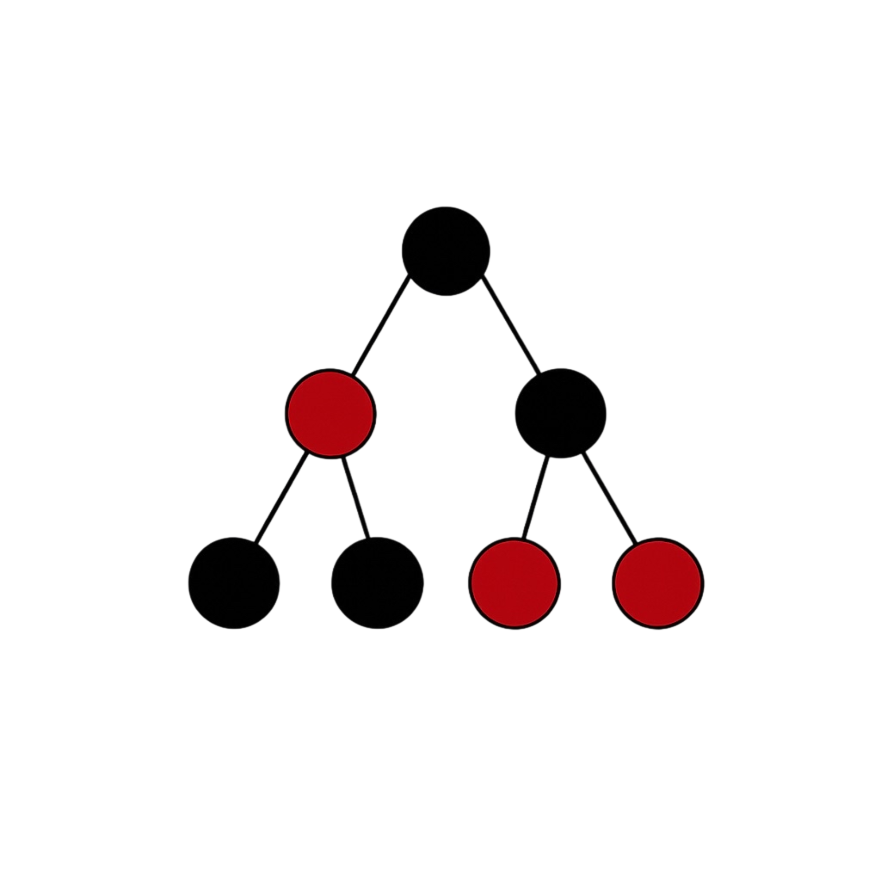
\includegraphics[width=0.38\paperwidth]{kcpc-logo.png}};
    \end{tikzpicture}%
}

\titleformat{\section}{\large\bfseries\color{kcpc-red}}{\thesection}{1em}{}

\setlist[itemize]{noitemsep, topsep=4pt}
\setlist[enumerate]{topsep=4pt}

\hypersetup{
    colorlinks=true,
    linkcolor=kcpc-red,
    urlcolor=kcpc-red
}

\title{KCPC Week 4 Problems\\Introduction to Graphs: Traversals, Structure, and Modelling}
\author{}
\date{}

\begin{document}

\maketitle
\thispagestyle{fancy}

\noindent
Welcome to Workshop 4 of the KCPC 2nd Semester series! This problem sheet accompanies the \textit{Introduction to Graphs} slides and is organised into three progressive sections:
\begin{itemize}
    \item \textbf{Section 1 --- Warm-Up Exercises:} Foundational applications of Breadth-First Search (BFS) and Depth-First Search (DFS) for connected components, unweighted shortest paths, cycle detection, and 2-colouring.
    \item \textbf{Section 2 --- Core Practice Exercises:} Structural graph properties including functional graphs, degree characterisations of cycles, dynamic programming on Directed Acyclic Graphs (DAGs), and tree diameter.
    \item \textbf{Section 3 --- Extended Homework:} Stretch competitive programming tasks requiring auxiliary bipartite graph construction and reverse sink-tree analysis on functional graphs.
\end{itemize}

\section{Warm-Up Exercises (Foundational Traversals)}

\subsection{Building Roads}
\textbf{Link:} \url{https://cses.fi/problemset/task/1666} \\
\textbf{Prerequisites:} Adjacency list representation, connected components via DFS or BFS.

Byteland has $n$ cities ($1 \le n \le 10^5$) and $m$ bidirectional roads ($1 \le m \le 2 \cdot 10^5$) connecting pairs of cities. The goal is to construct new roads so that there is a route between any two cities.

\textbf{Task:} Determine the minimum number of new roads required to make the entire road network connected, and output a valid list of roads $(u_i, v_i)$ to build.

\subsection{Message Route}
\textbf{Link:} \url{https://cses.fi/problemset/task/1667} \\
\textbf{Prerequisites:} Breadth-First Search (BFS), shortest unweighted paths, parent pointer reconstruction.

Syrj{\"a}l{\"a}'s network has $n$ computers ($2 \le n \le 10^5$) and $m$ undirected connections ($1 \le m \le 2 \cdot 10^5$). Uolevi wants to send a message from computer $1$ to computer $n$.

\textbf{Task:} Decide whether computer $n$ is reachable from computer $1$. If so, find the minimum number of computers along a valid route (including both endpoints $1$ and $n$) and print the sequence of computers on one such shortest route; otherwise, print \texttt{IMPOSSIBLE}.

\subsection{Round Trip}
\textbf{Link:} \url{https://cses.fi/problemset/task/1669} \\
\textbf{Prerequisites:} Depth-First Search (DFS), back-edges in undirected graphs, cycle reconstruction.

Byteland has $n$ cities ($1 \le n \le 10^5$) and $m$ bidirectional roads ($1 \le m \le 2 \cdot 10^5$). You want to design a round trip that begins in some city, passes through at least two other distinct cities, visits no intermediate city more than once, and returns to the starting city.

\textbf{Task:} Find any simple cycle of length at least $3$ in the undirected graph and print the number of vertices on the route (counting the start/end city twice, so $k \ge 4$) followed by the sequence of cities visited. If the graph is a forest (acyclic), print \texttt{IMPOSSIBLE}.

\subsection{Building Teams}
\textbf{Link:} \url{https://cses.fi/problemset/task/1668} \\
\textbf{Prerequisites:} Bipartite graphs, odd-cycle characterisation, 2-colouring via BFS or DFS.

There are $n$ pupils ($1 \le n \le 10^5$) in Uolevi's class and $m$ friendships ($1 \le m \le 2 \cdot 10^5$) between them. Your task is to divide the pupils into two teams (labelled $1$ and $2$) such that no two friends belong to the same team.

\textbf{Task:} Output a valid team assignment ($1$ or $2$) for each pupil $1, 2, \dots, n$, or print \texttt{IMPOSSIBLE} if the friendship graph is not bipartite.

\section{Core Practice Exercises (Structure, Trees, and DAGs)}

\subsection{Badge}
\textbf{Link:} \url{https://codeforces.com/contest/1020/problem/B} \\
\textbf{Prerequisites:} Directed graphs, functional graphs (out-degree $1$), cycle entry detection.

In a school of $n$ students ($1 \le n \le 1000$), whenever the teacher catches student $a$ playing a prank, a hole is punched in $a$'s badge and student $a$ blames student $p_a$ ($1 \le p_a \le n$). The teacher then moves to $p_a$, punches a hole in $p_a$'s badge, and continues following the chain $x \to p_x$ until reaching a student whose badge already has a hole (who then receives a second hole).

\textbf{Task:} For every possible starting student $a \in \{1, 2, \dots, n\}$, determine which student is the first to receive two holes in their badge.

\subsection{Cyclic Components}
\textbf{Link:} \url{https://codeforces.com/problemset/problem/977/E} \\
\textbf{Prerequisites:} Connected components, vertex degree invariants.

You are given an undirected simple graph with $n$ vertices ($1 \le n \le 2 \cdot 10^5$) and $m$ edges ($0 \le m \le 2 \cdot 10^5$). A connected component is a \textit{simple cycle} if its vertices can be ordered $v_1, v_2, \dots, v_k$ ($k \ge 3$) such that the edges in the component are precisely $(v_1, v_2), (v_2, v_3), \dots, (v_{k-1}, v_k), (v_k, v_1)$ and no others.

\textbf{Task:} Count how many connected components of the graph are simple cycles.

\subsection{DAG Number of Routes (Game Routes)}
\textbf{Link:} \url{https://cses.fi/problemset/task/1681} \\
\textbf{Prerequisites:} Directed Acyclic Graphs (DAGs), topological sorting, dynamic programming on DAGs.

A game has $n$ levels ($1 \le n \le 10^5$) connected by $m$ directed teleporters ($1 \le m \le 2 \cdot 10^5$). The teleporter network contains no directed cycles (it is a DAG).

\textbf{Task:} Calculate the total number of distinct routes from level $1$ to level $n$, modulo $10^9 + 7$.

\subsection{Longest Path}
\textbf{Link:} \url{https://atcoder.jp/contests/dp/tasks/dp_g} \\
\textbf{Prerequisites:} Directed Acyclic Graphs (DAGs), memoized DFS or topological order DP.

You are given a simple Directed Acyclic Graph (DAG) $G$ with $N$ vertices ($2 \le N \le 10^5$) and $M$ directed edges $x_i \to y_i$ ($1 \le M \le 10^5$).

\textbf{Task:} Find the length (number of edges) of the longest directed path in $G$.

\subsection{Tree Diameter}
\textbf{Link:} \url{https://cses.fi/problemset/task/1131} \\
\textbf{Prerequisites:} Tree properties (unique paths), Two-BFS / Two-DFS farthest-node theorem. \\
\textbf{Note:} Try solving it without dynamic programming.

You are given an undirected tree consisting of $n$ nodes ($1 \le n \le 2 \cdot 10^5$) and $n - 1$ edges. The \textit{diameter} of a tree is the maximum distance (number of edges) between any two nodes.

\textbf{Task:} Compute the diameter of the tree in $O(n)$ time using graph traversals alone (without subtree dynamic programming).

\section{Extended Homework (Advanced Graph Modelling)}

\subsection{Rudolf and Subway}
\textbf{Link:} \url{https://codeforces.com/contest/1941/problem/G} \\
\textbf{Prerequisites:} Auxiliary bipartite graph construction (star expansion), unweighted BFS.

A subway network has $n$ stations and $m$ bidirectional tracks ($\sum n, \sum m \le 2 \cdot 10^5$). Each track $(u_i, v_i)$ belongs to a subway line of colour $c_i$ ($1 \le c_i \le 2 \cdot 10^5$). Riding along any sequence of connected tracks of the \emph{same} colour costs $1$ ticket, and switching to a track of a different colour costs an additional ticket.

\textbf{Task:} Given a starting station $b$ and destination station $e$, find the minimum number of subway lines Rudolf must use to travel from $b$ to $e$ ($0$ if $b = e$).

\subsection{Game on Axis}
\textbf{Link:} \url{https://codeforces.com/problemset/problem/1787/D} \\
\textbf{Prerequisites:} Functional directed graphs, cycle detection, reversed sink-tree subtree sizes.

There are $n$ points $1, 2, \dots, n$ ($\sum n \le 2 \cdot 10^5$) on a number line, each with an integer jump offset $a_i$ ($-n \le a_i \le n$). A token starts at point $1$; whenever it is at $x \in [1, n]$, it jumps to $x + a_x$. The game terminates if the token jumps outside $[1, n]$, and runs forever if it enters a cycle. Before the game starts, you choose one index $i \in \{1, \dots, n\}$ and replace $a_i$ with an integer $y \in [-n, n]$.

\textbf{Task:} Count how many of the $n(2n + 1)$ possible pairs $(i, y)$ result in a game that terminates in a finite number of steps.

\vspace{0.5em}
\begin{center}
    \textit{Full worked proofs, complexity analyses, and implementations in Python and C++ are provided in \textbf{Week 4 Solutions.pdf}.}
\end{center}

\end{document}
